\documentclass{standalone}
\usepackage[dvipsnames,svgnames,x11names]{xcolor}
\usepackage{tikz}
\usepackage{pgfplots}
\pgfplotsset{compat = 1.12}
\usepackage{../thesismath}
\begin{document}
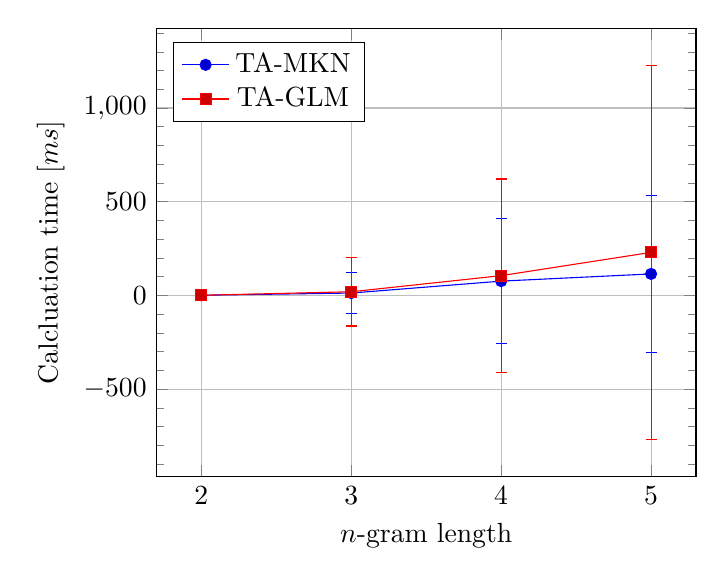
\begin{tikzpicture}[baseline]

\begin{axis}[
  xlabel = {$n$-gram length},
  xtick = {2, ..., 5},
  ylabel = {Calcluation time [$m s$]},
  minor y tick num = 4,
  grid = major,
  legend entries = {{TA-MKN}, {TA-GLM}},
  legend pos = north west,
]

% over 100 test sequences on my own machine

% TA-MKN
\addplot+[
  error bars/.cd,
  y dir = both,
  y explicit,
] table [y error = us_error] {
  n us       us_error
  2    0.880    4.054
  3   12.596  109.800
  4   76.195  332.309
  5  114.599  419.357
};

% TA-GLM
\addplot+[
  error bars/.cd,
  y dir = both,
  y explicit,
] table [y error = us_error] {
  n us       us_error
  2    0.686    3.694
  3   19.438  182.884
  4  105.366  515.740
  5  229.566  996.888
};

\end{axis}

\end{tikzpicture}
\end{document}
